\documentclass[12pt, a4paper]{report}
% for guidance, see phd_work/mnras_guide.pdf
%\setlength\parindent{0pt}

\usepackage[english]{babel}
\usepackage[utf8x]{inputenc}
\usepackage[T1]{fontenc}

%\documentclass[useAMS,usenatbib]{mn2e}
\newcommand{\aap}{A\&A}
\newcommand{\araa}{ARAA}
\newcommand{\mnras}{MNRAS}
\newcommand{\apjl}{ApJL}
\newcommand{\apjs}{ApJS}
\newcommand{\apj}{ApJ}
\newcommand{\aj}{ApJ}
\newcommand{\nat}{Nature}
\newcommand{\pasa}{PASA}
\newcommand{\pasj}{PASJ}
\newcommand{\pasp}{PASP}
\newcommand{\aapr}{A\&AR}
\newcommand{\procspie}{Proc. SPIE}
\newcommand{\apss}{Ap\&SS}
%\newcommand{\rsquo}{`}

\usepackage{graphicx}
%\usepackage{braket}
\usepackage[english]{babel}
\usepackage{upgreek}
\usepackage{graphicx}
\usepackage{float}
\usepackage{natbib}
\usepackage{amsmath}
\usepackage{amssymb}
\usepackage{tabularx,ragged2e,booktabs,caption}
\usepackage{graphicx} % for images
\usepackage[font=small]{caption}
\usepackage{setspace}
\usepackage{epstopdf}
\usepackage{subcaption}
\usepackage{url}

% ALW edit: FORMAT FOR INCLUDING PDF IMAGES!!!
% for guidance, see phd_work/grfguide.pdf
%\includegraphics[<options>]{filename.pdf}


%%%%%%%%%%%	Page layout settings that follow JMU regulations     %%%%%%%%%%

\setlength{\hoffset}{0mm}
\setlength{\oddsidemargin}{0mm}
\setlength{\evensidemargin}{0mm}

\setlength{\voffset}{-10mm}
\setlength{\topmargin}{0mm}
\setlength{\headheight}{10mm}
\setlength{\headsep}{10mm}

\setlength{\textheight}{220mm}
\setlength{\textwidth}{155mm}

\setlength{\columnsep}{10mm}
\setlength{\marginparsep}{0mm}
\setlength{\marginparwidth}{0mm}
\setlength{\footskip}{20mm}

\setlength{\parindent}{0.3in} % Size of indent at the start of a new paragraph - originally 0.0in
\setlength{\parskip}{0.0in} % Spacing between paragraphs - originally 0.1in

\usepackage[hang,splitrule]{footmisc}

\addtolength{\footskip}{0.5cm}
\setlength{\footnotemargin}{0.3cm}
\setlength{\footnotesep}{0.4cm}

\makeatletter
\let\splitfootnoterule=\pagefootnoterule
\makeatother



\begin{document}

\chapter{Introduction}
\section{Motivation}

Stellar populations, most prominently star clusters, represent one of the richest sources of information in the known universe. Stars within clusters are generally believed to have formed in a single brief time-period, making their ages essentially the same. Furthermore, because the stars are clustered in the night sky, the regions of space through which the light from each star travels to reach the same telescope are far more likely to be very similar to the relevant regions for all the other cluster stars, meaning the effects of the interstellar environment on the light is more likely to be the same for all the stars. This greatly simplifies the observational corrections required to analyse the physics of the cluster and the individual stars. This allows for direct comparison with current theoretical models, allowing detailed study of the physics stellar magnetic fields, rotation and internal mixing, among others. Determining the age of a cluster is an extremely powerful tool for this, especially for stars too far away to observe their physical properties with high precision.**** ****understanding of galactic history, elemental abundances, etc.

As the light emitted from a star travels towards a distant observer, its intensity, or flux, $F$ decreases with distance $d$ via an inverse-square law:

\begin{equation}
\label{flux_def}
F = \frac{L}{4 \pi d^{2}}
\end{equation}

where $L$ is the star's luminosity, which is an intrinsic property of the star (i.e., independent of the observer). Equation \ref{flux_def} is a natural consequence of the same light wave expanding outwards from its source into a progressively larger spherical volume of empty space.

However, the interstellar medium is not a perfect vacuum. It contains many different structures, such as diffuse gas clouds, that can absorb or scatter light passing through, depending on the wavelength of the incoming photons, the spacing between the individual atoms (i.e.,the density of the medium) and the quantum levels in the atoms occupied by their electrons. These absorption and scattering events are known as interstellar extinction. For a given source, its interstellar extinction coefficient represents the sum of the effects of all extinction events along the line-of-sight between the source and the observer.

Interstellar extinction preferentially affects light at shorter (i.e., bluer) wavelengths. Therefore, the effect of extinction is sometimes referred to as ``reddening'', despite the fact that this term is also applied to a related, but distinct, quantity (see Section \ref{extinc_desc}). Therefore, it should be expected that sources with proportionally higher fluxes at shorter wavelengths are most affected by extinction.

The goal of this project is to attempt to use analytic functions to model the variation of the extinction coefficients in multiple filter systems, across as large a range of stellar types as possible, with the ultimate goal of using this simplification of the variations to determine the differences in the estimated optimal ages, elemental abundances (known collectively in astronomy as metallicity) and ****$A_{V}$ values of stellar populations (i.e., star clusters) from the current standard method for simulating extinction. If such differences exist and if they are of significant size, it could cause a recalculation of the properties of observed star clusters.

Because star clusters are mostly composed of stars that formed from the same molecular gas cloud in a very short time period This could potentially cause a reinterpretation of these clusters' history, including where and when they formed in the Milky Way and the chemical enrichment of the gas that formed their stars.

\section{Observational constraints}
No telescope can view the sky at all spectral wavelengths - it would be wholly impractical due to the sheer number of sources across the spectrum, as well as the fact that telescope resolution depends on the wavelength of the incoming light. Therefore, modern telescopes are equipped with a system of filters or bands, which allow only light within a narrow range of wavelengths. In a filter system, the individual filters are designed to operate best at different wavelengths. The system will be therefore have the following properties:

\begin{itemize}
\item the filters cover a much wider range of spectral wavelengths than a single filter would alone; this is used to observe sources at different wavelengths to determine its spectral colour **** (see Section ****).
\item The filters are designed such that the range of wavelengths in which they can best detect incoming light overlap with their neighbours, as shown in Figures \ref{Gaia_response_funcs}-\ref{ACS_response_funcs}. This ensures that there are no wavelength gaps in which incoming light cannot be detected. This is particularly important for quantum line emission, which occurs only at specific wavelengths for particular electron occupancy levels (see Section**** for exceptions relevant to this case). One of the most prominent case of astrophysical line emission is that of H$\alpha$, in which the electron in a neutral hydrogen atom transitions from the $n = 3$ to the $n = 2$ quantum occupation state, emitting a photon with a wavelength of 656 nm, which is in the red part of the visible spectrum.
\end{itemize}

****Filters - Johnson, ACS, WFC/UVIS, Gaia

\begin{figure}[h]
\begin{center}
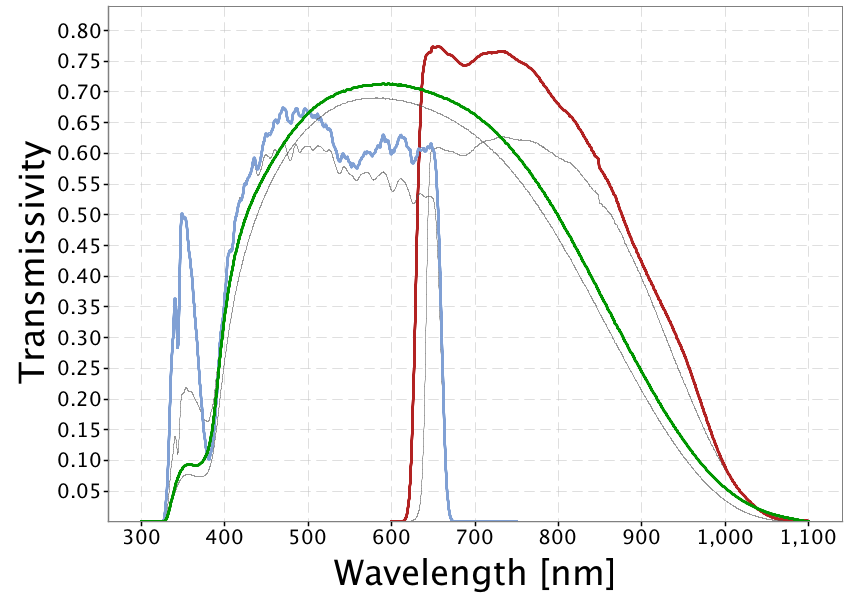
\includegraphics[scale=0.5]{GaiaDR2Passbands.png}
\caption{Filter response functions for Gaia photometric filters. Source: \protect\url{https://www.cosmos.esa.int/web/gaia/iow_20180316}}
\label{Gaia_response_funcs}
\end{center}
\end{figure}

\begin{figure}[h]
\begin{center}
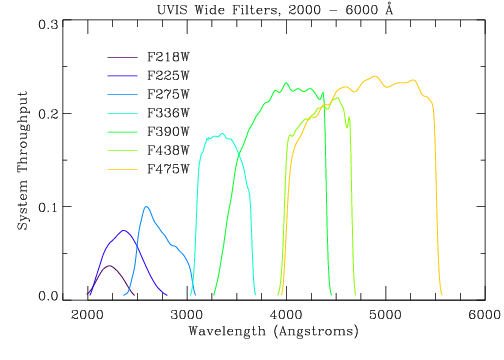
\includegraphics[scale=0.5]{UVIS_Wide1.jpg}
\caption{Filter response functions for wide-field WFC3 filters. Source: \protect\url{http://www.stsci.edu/hst/wfc3/ins_performance/throughputs/UVIS_filterthru.html}}
\label{WFC3_response_funcs1}

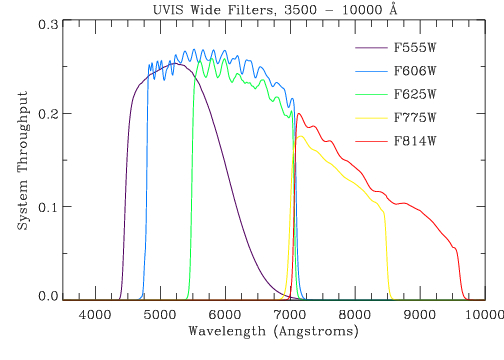
\includegraphics[scale=0.5]{UVIS_Wide2.jpg}
\caption{Filter response functions for wide-field WFC3 filters. Source: \protect\url{http://www.stsci.edu/hst/wfc3/ins_performance/throughputs/UVIS_filterthru.html}}
\label{WFC3_response_funcs2}

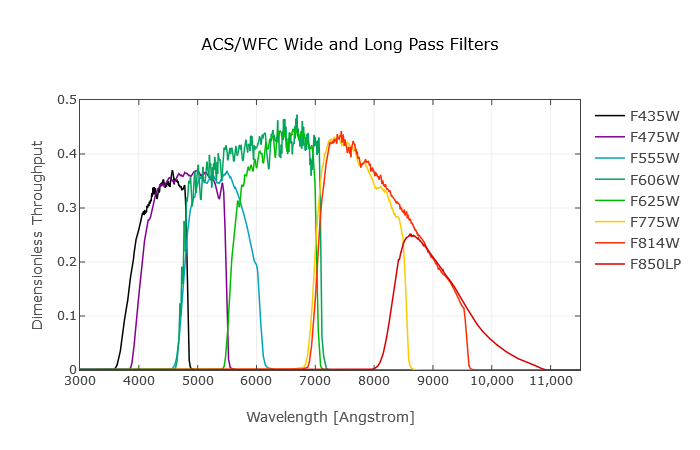
\includegraphics[scale=0.5]{ACS_Wide.png}
\caption{Filter response functions for wide-field ACS filters. Source: \protect\url{http://www.stsci.edu/hst/acs/analysis/throughputs}}
\label{ACS_response_funcs}
\end{center}
\end{figure}

The standard treatment of extinction is to apply a single constant value of the extinction coefficient for a given filter $X$, denoted in the literature by $A_{X}$. For wavelengths in or close to the optical spectral range, this quantity is usually expressed as a fixed ratio of the (constant) coefficient value in the Johnson-$V$ filter, the standard visual comparison filter.

In this project, three broad-band filter systems were employed. These are the Advanced Camera for Surveys (ACS) and the Ultraviolet Imaging Spectrograph channel of the Wide-Field Camera 3 (WFC3/UVIS), both mounted on the Hubble Space Telescope (HST), and the single set of three broadband filters mounted on the Gaia space observatory \citep{2010A&A...523A..48J}.

\begin{table}
\begin{center}
\begin{tabular}{cccccc}
\hline
System & Filter & Central wavelength / \AA & FWHM / \AA \\
\hline
& F435W & 4760 & 729 \\
& F475W & 5000 & 986 \\
& F555W & 5060 & 841 \\
ACS & F606W & 6690 & 1566 \\
& F625W & 6480 & 978 \\
& F775W & 7320 & 1017 \\
& F814W & 7460 & 1657 \\
\hline
& F218W & 2175 & 300 \\
& F225W & 2250 & 500 \\
& F275W & 2750 & 500 \\
& F300X &  & 2775 \\
& F336W & 3375 & 550 \\
& F390W & 3900 & 1000 \\
WFC3 & F438W & 4320 & 695 \\
& F475W & 4750 & 1520 \\
& F555W & 5410 & 1605 \\
& F606W & 5956 & 2340 \\
& F625W & 6250 & 1550 \\
& F775W & 7760 & 1470 \\
& F814W & 8353 & 2555 \\
\hline
& G & 6730 & 4400 \\
Gaia & G\textsubscript{bp} & 5320 & 2530 \\
& G\textsubscript{rp} & 7970 & 2960 \\
\hline

\end{tabular}
\caption{Basic properties of the filters employed in this project.}
\label{filter_basics}
\end{center}
\end{table}

Filters thus**** present a challenge when trying to determine stellar spectra accurately. This task is further complicated by the fact that, even in the wavelength range where a filter does detect incoming flux, the fraction of light it detects, known as the transmittance, is not uniform across the range. The transmittance as a function of wavelength is known as a transmission curve, bandpass or filter response function. Examples of response functions for some**** of the filters employed in this project are shown in Figure \ref{ACS_response_funcs}. By comparing these with the filters' information in Table \ref{filter_basics}, it can be seen that the exact shape of the response function could have a significant impact on the observed spectrum if not taken into account.
The values in the column labelled 'FWHM' represents the full width at half-maximum. In this case, it is defined as the difference between the lowest and highest wavelength values at which the transmittance value is half of its maximum value for the filter, typically assuming the response function can be approximated as a Gaussian distribution centred on the central wavelength. The FWHM acts as an approximate measure of the wavelength range within which the filter can reliably be used for observations.

The wavelengths of light visible to an average human eye are in the range 3800-7400 \AA . Hence, the filters used here cover wavelengths from the soft-ultraviolet (soft-UV) to the near-infrared (NIR),  including all visible wavelengths.

\section{Basics of stellar evolution} \label{stel_evol}
While observations can reveal properties of individual stars and stellar populations more generally, the significance of these properties can only be gained by understanding the underlying physical processes and structure of the stars themselves.

****It can be seen that all stars lie on a single, complicated line, known as an isochrone. Isochrones for different population ages and metallicities are calculated using theoretical stellar models for the largest possible spread of initial stellar masses. An isochrone in the HR diagram has a number of distinct features:
\begin{itemize}
\item Most stars, including the coolest and least-luminous ones, follow a tight pattern of luminoaity increasing with temperature. This is known as the main sequence (MS)
\item This pattern stops as the luminosity continues to increase slowly but with decreasing temperature. The end of the MS is called the main-sequence turn-off (MSTO), which is followed by the sub-giant branch (SGB).
\item After the SGB, the gradient becomes much steeper, with temperate decreasing and luminosity rapidly increasing. This is the red-giant branch (RGB).
\item At the tip of the RGB, stars start becoming fainter and their temperatures increase. Eventually, their is a sequence of stars with near-constant luminosity but a range of effective temperatures. This is the horizontal branch (HB).
\item After the horizontal branch, there is again a rapid increase in luminosity accompanied by a slow decrease in temperature. This is the asymptotic giant branch (AGB).
\end{itemize}

In the main sequence, nuclear fusion occurs in the core and any products must be subjected to mixing effects to reach the atmosphere. Since stellar interiors are physically fluid, heavier nuclei, which are more dense, preferentially gather in regions close to the star's centre of gravity. Therefore, processes such as convection, thermohaline mixing and radiative levitation are required to induce a noticeable change in surface composition. However, these processes require certain physical conditions on local scales, if they are to be sustained for long enough to induce a visible change in the stellar spectrum.

On the main-sequence, only low-mass stars ($M_{*} \lesssim 0.38M_{\odot}$) \citep{2018A&A...619A.177B} have fully-convective interiors. Massive ($M_{*} \gtrsim 1.5M_{\odot}$) stars have convective cores, but radiative envelopes. Intermediate-mass stars, including the Sun, have radiative cores and convective envelopes. Since regions in which energy transport is dominated by radiative effects are stable against convection, stars with masses greater than $0.38M_{\odot}$ are highly unlikely to show large changes in atmospheric composition along the main sequence. However, the fully-convective lower-mass stars are able to do so. Therefore, the faintest and reddest parts of the main sequence are most likely to have atmospheres enriched with metals, which would be confined in the cores of more massive stars. These enriched atmospheres are therefore highly sensitive to the overall metallicity of the original gas cloud in which the star, and its parent cluster if applicable, formed.

It should be noted that the estimated position of the MSTO of an isochrone in the HR diagram is not only a reflection of the isochrone age, but also of the internal stellar physics. This can include not only the deactivation of core-hydrogen fusion but also smaller effects, including the strength of the convective core overshooting in sufficiently massive stars, which is particularly useful for younger open clusters \citep{2004PASP..116..997V}.

\begin{equation}
\nabla_{\textnormal{rad}} = \frac{3\kappa LP}{16\pi acGmT^{4}}
\end{equation}

To illustrate, let us consider a bubble of gaseous material in pressure-equilibrium with its surroundings and represent mixing as a significant change in the bubble's (radial) position on a significant time-scale, arising from small differences in the remaining 3 thermodynamic quantities between the bubble and its surroundings. For a non-rotating star, using a simple linear approach, together with the Archimedes principle, gives a set of 4 homogeneous differential equations for the (small) differences in $P$, $T$, $\mu$ and $r$ (Equations (3.1)-(3.4) in \cite{2017RSOS....470192S}). If $\Delta x_{i}$ are the differences in the 4 parameters, taking the ansatz form $\Delta x_{i} = B_{i} e^{nt}$ allows for a solution as a 3rd-order polynomial in $n$ (Equation (3.5) in \cite{2017RSOS....470192S}), if the determinant of the relevant matrix (dependent of the values of the $B_{i}$) is zero. The Routh-Hurwitz stability criterion can then be applied to this polynomial to give a general solution for $n$. For a physically-unstable solution, the exponent in the $\Delta x_{i}$ equation must be positive, i.e. $n$ must satisfy the condition $\operatorname{Re}(n) > 0$. Hence, the subsequent constraints on the polynomial coefficients form all the possible conditions for instability,  of which at least one must be satisfied. These constraints take the following form:

\begin{align}
\nabla _{\mu} &< 0 \label{mu_inv_ineq} \\
\nabla _{\textnormal{rad}} &> \nabla _{\textnormal{ad}} \label{schwarz_ineq} \\
\nabla _{\textnormal{rad}} &> \nabla _{\textnormal{ad}} + \left( \frac{\phi}{\delta} \right) \nabla _{\mu} \label{ledoux_ineq}
\end{align}

where $\nabla _{\mu} = d\ln\mu / d\ln P$, $\nabla _{\textnormal{rad}} = \left(\partial\ln T / \partial\ln P \right)_{\textnormal{rad}}$ and $\nabla _{\textnormal{ad}} = \left(\partial\ln T / \partial\ln P \right)_{\textnormal{ad}}$ are the temperature-pressure gradients for the local environment (dominated by radiation pressure) and the bubble (treated as an adiabatic ideal gas), respectively, $\phi = \left( \partial \ln\rho / \partial \ln\mu \right)_{P,T}$ and $\delta = -\left( \partial \ln\rho / \partial \ln T \right)_{P,\mu}$  \citep{1980A&A....91..175K}.

In stellar evolution, the stages described in **** represent extended periods of time in which the stellar interior, described in theoretical models as a series of (quasi-)spherical shells, can be described as being in hydrostatic equilibrium, i.e., the gravitational pressure inwards on material in a given shell, due to the mass enclosed by the shell, is equal to the radiation pressure outwards generated by nuclear fusion occurring within the area enclosed by the shell, either in the core or in an inner shell. Giant stars are objects with luminosities significantly higher and surface gravities lower than stars on the main sequence (which generally have gravities in the range 4 $\lesssim$ log($g$) $\lesssim$ 5.5).

\section{Previous studies}
\cite{1989ApJ...345..245C} used observations of bright main-sequence stars to produce empirical equations describing the ratio of extinction coefficients at a specific wavelength $\lambda$ ($A_{\lambda}$) and the Johnson-$V$ filter ($A_{V}$), respectively. From this point onward, this ratio will be referred to as $A_{\lambda}/A_{V}$. They produced a basic universal equation of the form:

% avoided the complications of using reddening (which is not itself intrinsic and whose implications be impacted by the choice of filters) by 

\begin{equation}
A_{\lambda}/A_{V} = a(x) + b(x)/R_{V},
\label{CCM_general}
\end{equation}

where $x \equiv 1/\lambda$ and $R_{V} \equiv A(V)/E(B-V)$. The significance of $R_{V}$, as noted in the same paper, comes from its usefulness as an indicator of the nature of the interstellar medium through which the observed light travels in order to reach the observer.**** The total wavelength range was divided into 4 sub-ranges, each with a governing pair of empirically-determined equations (to determine $a(x)$ and $b(x)$, respectively). The CCM89 model underpins more recent studies of intrinsic effects on extinction (\cite{2008PASP..120..583G}, \cite{2018MNRAS.479L.102C}), and provides the basis for the synthetic $A_{X}/A_{V}$ datasets in this project, ****where $A_{X}$ is the coefficient for a given filter $X$.

\cite{2008PASP..120..583G} produced data tables of $A_{X}/A_{V}$ via bolometric corrections (as was carried out in this study). for stellar atmosphere models with parameters $T_{\textnormal{eff}}$, log($g$) and [Fe/H]. They carried this out using the same ATLAS9 data that was used to generate the data for this project, but also combining it with data from other studies**** \cite{2002A&A...391..195G}, resulting in data covering a parameter space extending beyond the ATLAS9 limits in all three parameters. They used the data tables to directly calculate the $A_{X}/A_{V}$ values for the stellar models in theoretical isochrones. While determining that the values of $A_{X}/A_{V}$ varied significantly with $T_{\textnormal{eff}}$ and log($g$), the variation with metallicity was found to be ~0.17$\%$ between [Fe/H] = 0.0 and [Fe/H] = -2.5. They found that, when they set $A_{V} = 6$, there was a systematic shift for the ACS system between extinction values calculated star-wise using the BC tables and a constant extinction value. The constant values of $A_{X}/A_{V}$ were calculated from a yellow dwarf in the low-extinction regime. Overall, the BC tables produced a smaller extinction coefficient in the F814W filter and a larger (F475W-F814W) colour index value. It also caused a change in the shape of the curve at the MSTO. They then applied the BC table data method to the case of the globular cluster M92. They found the optimal metallicity to be $Z = 0.0004$ ([Fe/H] $\approx$ -1.6) instead of the value obtain by previous observers of $Z = 0.0001$ ([Fe/H] $\approx$ -2.2). Therefore, their use of BC data caused the estimated cluster metallicity to be greater than when using the standard one-size-fits-all approach to extinction.

\cite{2018MNRAS.475.5023C}, using bolometric correction tables the same authors calculated in a previous study \citep{2014MNRAS.444..392C} from MARCS atmospheric models \citep{2008A&A...486..951G}, created and fitted simple linear models in the Hipparcos/Tycho, Pan-STARRS1, SkyMapper, and JWST filter systems, expressed for $R_{X}  = \frac{A_{X}}{E(B-V)}$. The equation is independent of surface gravity and has the following form:

\begin{equation}
R_{X}  = a_{0} + T_{4}(a_{1} + a_{2}T_{4}) + a_{3}\textnormal{[Fe/H]}
\label{casagrande_ext_fit}
\end{equation}

where $T_{4} = 10^{-4} \times T_{\textnormal{eff}}$. The equation is valid for $5250\textnormal{K} \leq T_{\textnormal{eff}} \leq 7000\textnormal{K}$ and $\leq \textnormal{[Fe/H]}$. It was calculated using a surface gravity of log($g$) = 4.1. In their latest paper utilising Equation \ref{casagrande_ext_fit}\citep{2018MNRAS.479L.102C}, the authors applied the same approach to  the three wide-field Gaia filters.

There are key differences between that project and the one presented here, however. Firstly, \citep{2014MNRAS.444..392C} used MARCS model atmospheres instead of ATLAS9, with MARCS models restricted to effective temperatures lower than 8000K. More importantly, the ranges in metallicity and, in particular, effective temperature covered by the model in Equation \ref{casagrande_ext_fit} were smaller than the ones covered in this project. This makes the results of this project more applicable for a wider range of $T_{\textnormal{eff}}$ values and therefore stellar population ages, particularly for very young open clusters.


\bibliographystyle{mnras} % unsrtnat
\bibliography{mphil_thesis}

\end{document}